\documentclass[./project-report/src/latex/project-report.tex]{subfiles}

\begin{document}

\maketitle

\section{Technical Solution TODO}

\subsection{Setup}

\subsubsection{File Structure}

I used the following file structure to organise the code for the project, where school\_project is the main package and is constructed of two main subpackages:

\begin{itemize}
    \item The models package, which is a self-contained package for creating trained Artificial Neural Network models.
    \item The frames package, which consists of tkinter frames for the User Interface.
\end{itemize}

\pagebreak

\begin{footnotesize}
\verbatiminput{|"git ls-tree -r --name-only HEAD | grep -v -E 'project-report/|Makefile' | tree --fromfile --charset=ascii"}
\end{footnotesize}

\pagebreak

Each package within the school\_project package contains a \_\_init\_\_.py file, which allows the school\_project package to be installed to a virtual environment 
so that the modules of the package can be imported from the installed package.

\begin{itemize}
    \item Here is the contents of the frames package's \_\_init\_\_.py for example, which allows the classes of all modules in the package to be imported at once:
        \inputminted{python}{./school_project/frames/__init__.py}
\end{itemize}

I have omitted the source code for this report, which included a Makefile for its compilation.

\subsubsection{Dependencies}

The python dependencies for the project can be installed simply by running the following setup.py file (as described in the README.md in the next section). Instructions on 
installing external dependencies, such as the CUDA Toolkit for using a GPU, are explained in the README.md in the next section also.

\begin{itemize}
    \item setup.py code:
        \inputminted{python}{./setup.py}
\end{itemize}

\subsubsection{Git and Github files}

To optimise the use of Git and GitHub, I have used the following files:

\begin{itemize}
    \item A .gitignore file for specifying which files and directories should be ignored by Git:
        \inputminted{text}{./.gitignore}
    \item A README.md markdown file to give installation and usage instructions for the repository on GitHub:
        \begin{itemize}
            \item Markdown code:
                \inputminted{markdown}{./README.md}
            \item Which will generate the following:
                \begin{figure}[h!]
                \centering
                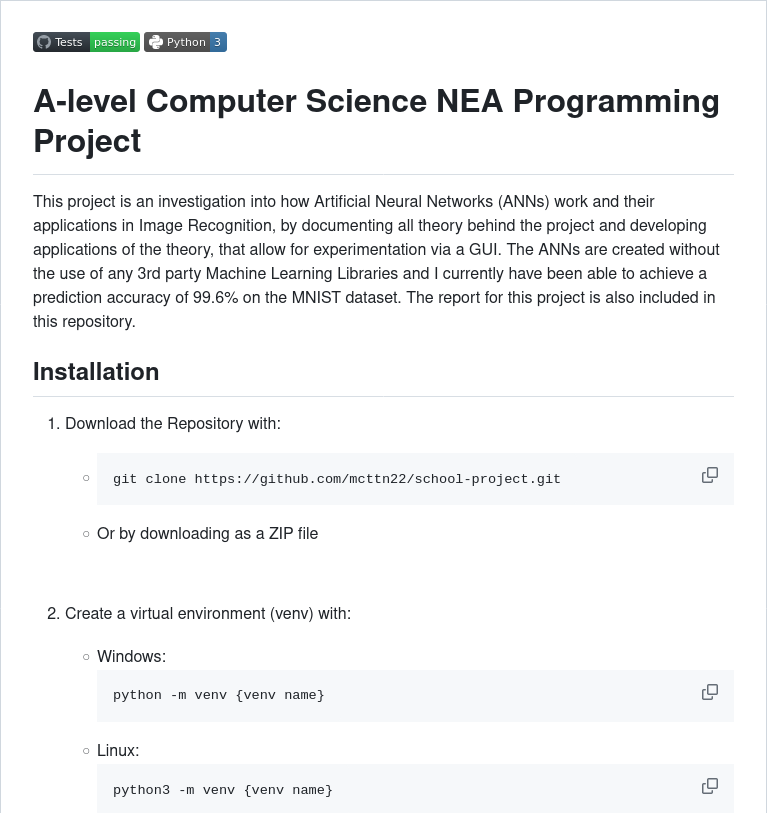
\includegraphics[width=1\textwidth]{./project-report/src/images/readme-top.png}
                \end{figure}
                \pagebreak
                \begin{figure}[h!]
                \centering
                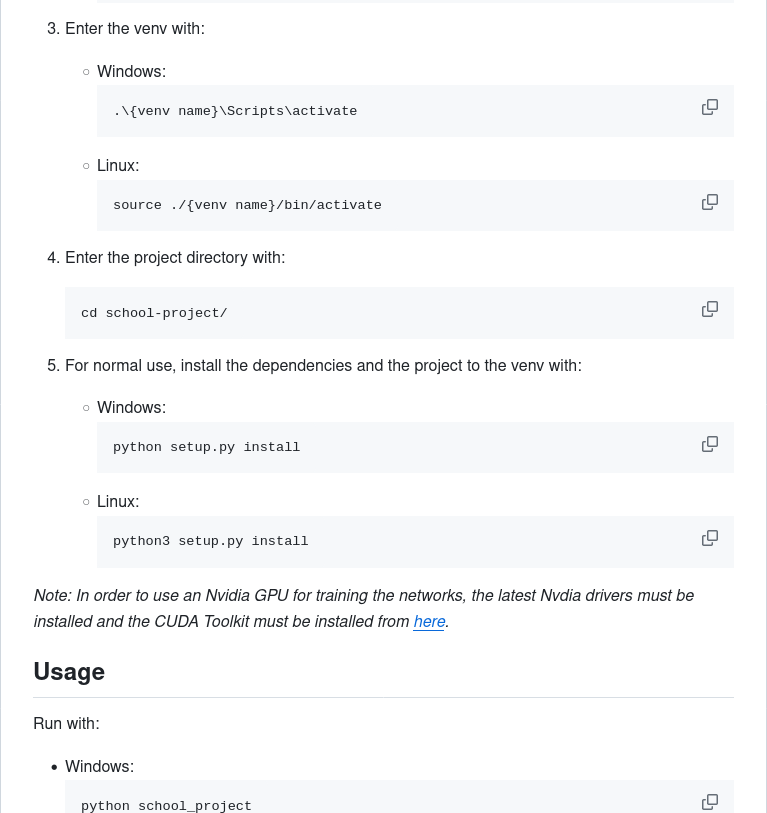
\includegraphics[width=1\textwidth]{./project-report/src/images/readme-middle.png}
                \end{figure}
                \pagebreak
                \begin{figure}[h!]
                \centering
                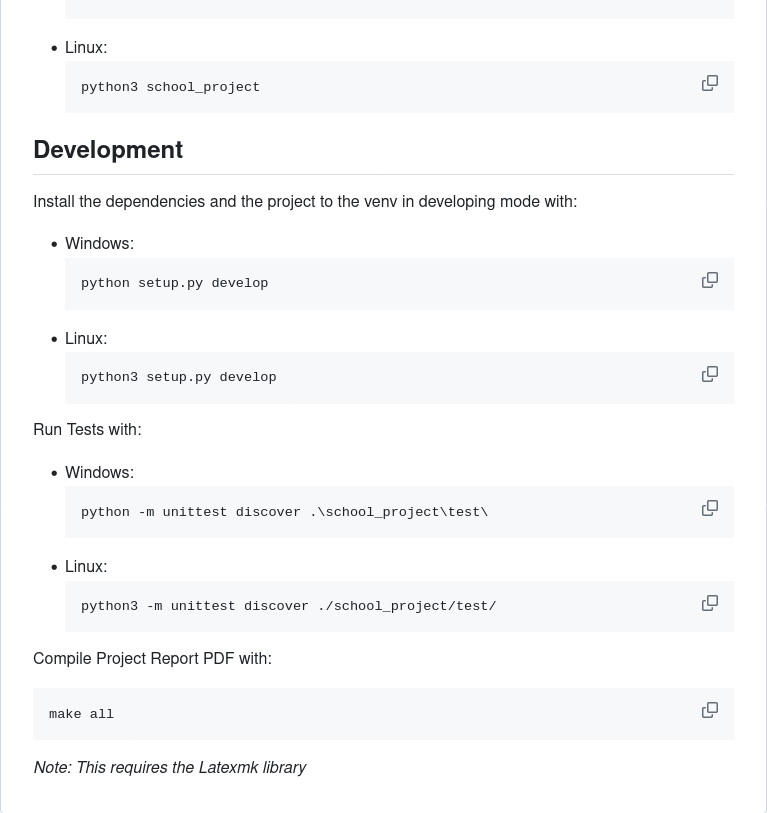
\includegraphics[width=1\textwidth]{./project-report/src/images/readme-bottom.png}
                \end{figure}
        \end{itemize}
    \item A LICENSE file that describes how others can use my code.
\end{itemize}

\subsubsection{Organisation}

I also utilise a TODO.md file for keeping track of what features and/or bugs need to be worked on.

\subsection{models package}

This package is a self-contained package for creating trained Artificial Neural Networks and can either be used for a CPU or a GPU, as well as containing the test 
and training data for all three datasets in a datasets directory. Whilst both the cpu and gpu subpackage are similar in functionality, the cpu subpackage uses NumPy 
for matrices whereas the gpu subpackage utilise NumPy and another library CuPy which requires a GPU to be utilised for operations with the matrices. For that reason 
it is only worth showing the code for the cpu subpackage.

Both the cpu and gpu subpackage contain a utils subpackage that provides the tools for creating Artificial Neural Networks, and three modules that are the implementation 
of Artificial Neural Networks for each dataset.

\subsubsection{utils subpackage}

The utils subpackage consists of a tools.py module that provides a ModelInterface class and helper functions for the model.py module, that contains an AbstractModel 
class that implements every method from the ModelInterface except for the load\_dataset method.

\begin{itemize}
    \item tools.py module:
        \inputminted{python}{./school_project/models/cpu/utils/tools.py}
    \item model.py module:
        \inputminted{python}{./school_project/models/cpu/utils/model.py}
\end{itemize}

\subsubsection{Artificial Neural Network implementations}

The following three modules implement the AbstractModel class from the above model.py module from the utils subpackage, on the three datasets.

\begin{itemize}
    \item cat\_recognition.py module:
        \inputminted{python}{./school_project/models/cpu/cat_recognition.py}
    \item mnist.py module:
        \inputminted{python}{./school_project/models/cpu/mnist.py}
    \item xor.py module
        \inputminted{python}{./school_project/models/cpu/xor.py}
\end{itemize}

\subsection{frames package}

I decided to use tkinter for the User Interface and the frames package consists of tkinter frames to be loaded onto the main window when needed. The package also 
includes a hyper-parameter-defaults.json file, which stores optimum default values for the hyper-parameters to be set to.

\begin{itemize}
    \item hyper-parameter-defaults.json file contents:
        \inputminted{json}{./school_project/frames/hyper-parameter-defaults.json}
    \item create\_model.py module:
        \inputminted{python}{./school_project/frames/create_model.py}
        
        Which outputs the following for the hyper-parameter frame:

        \pagebreak
        
        \begin{figure}[h!]
        \centering
        \frame{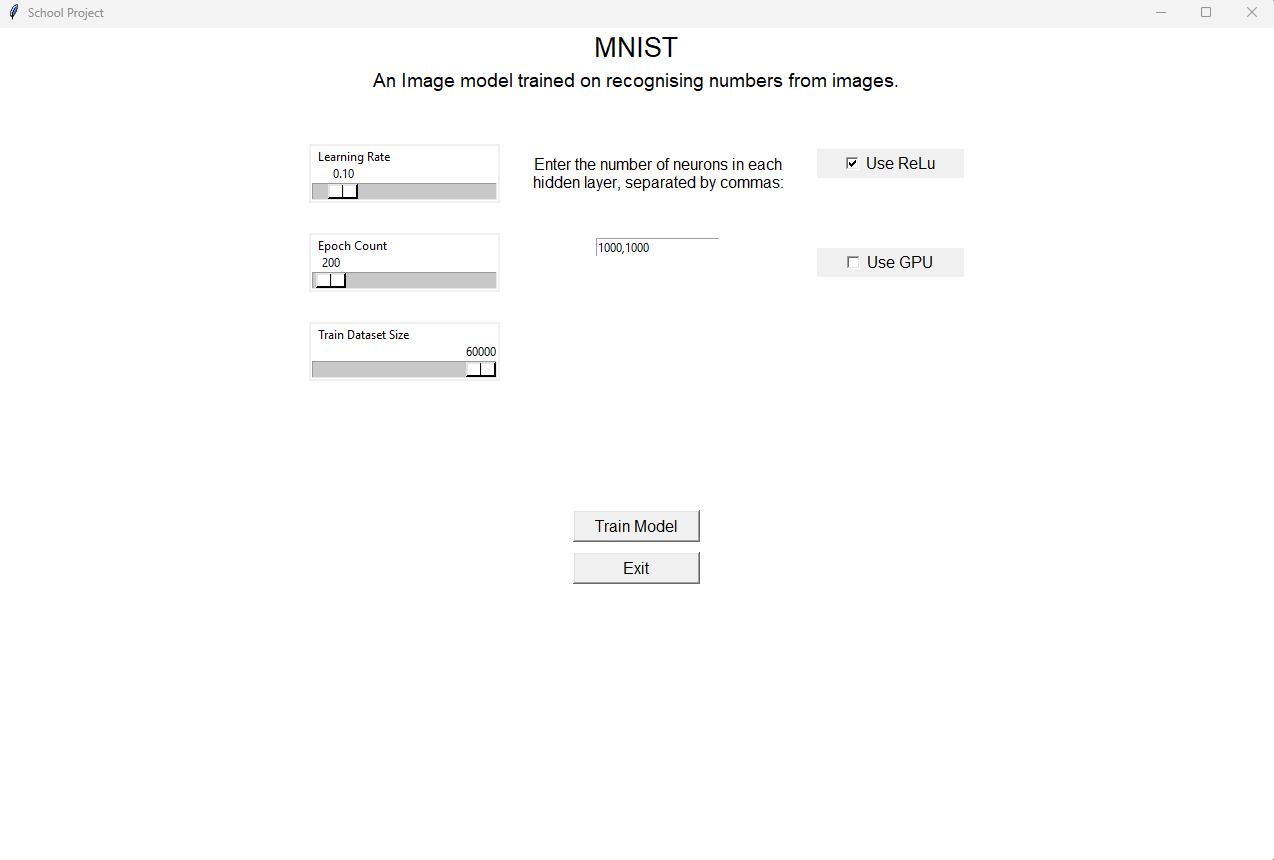
\includegraphics[width=1\textwidth]{./project-report/src/images/hyper-parameter-frame.png}}
        \end{figure}

        And outputs the following for the training frame during training:

        \begin{figure}[h!]
        \centering
        \frame{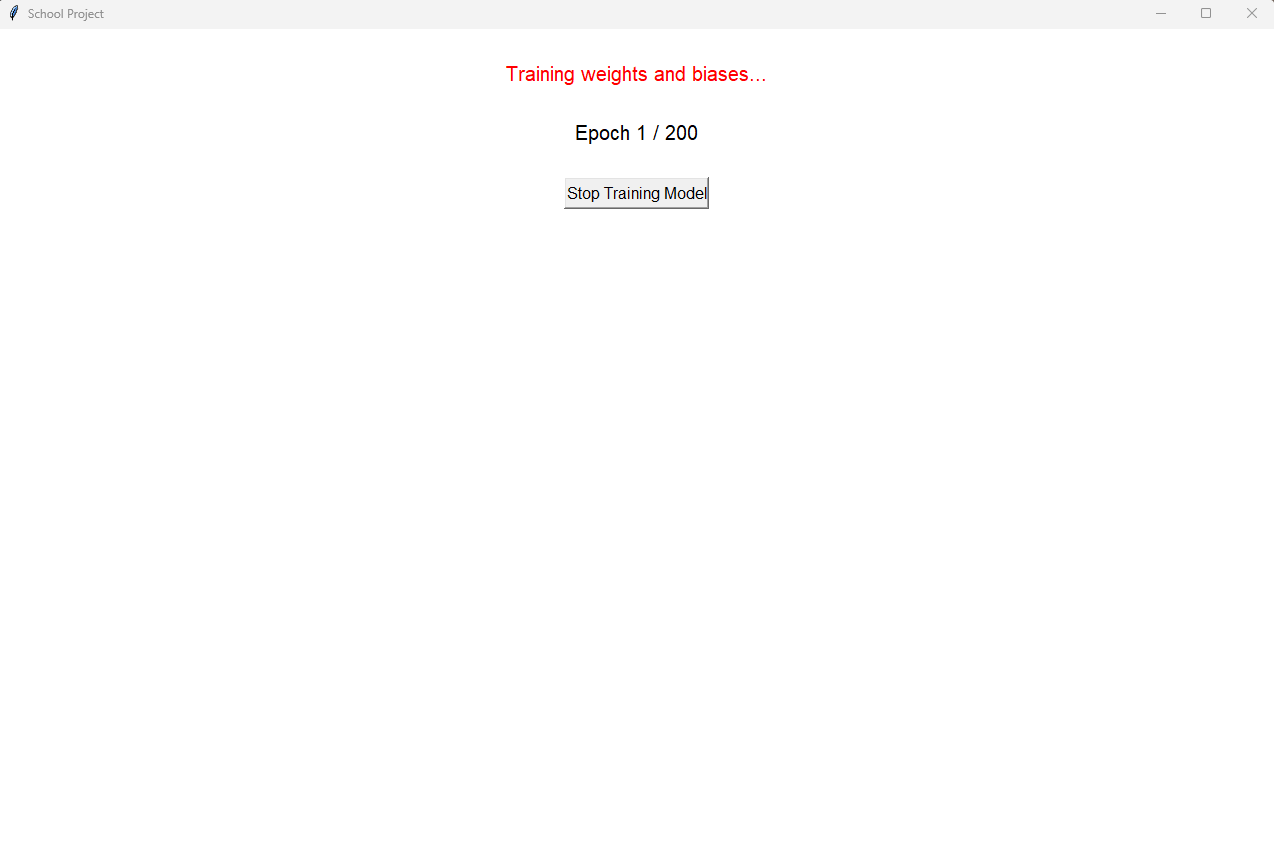
\includegraphics[width=1\textwidth]{./project-report/src/images/training-frame-1.png}}
        \end{figure}

        \pagebreak

        And outputs the following for the training frame once training has completed:

        \begin{figure}[h!]
        \centering
        \frame{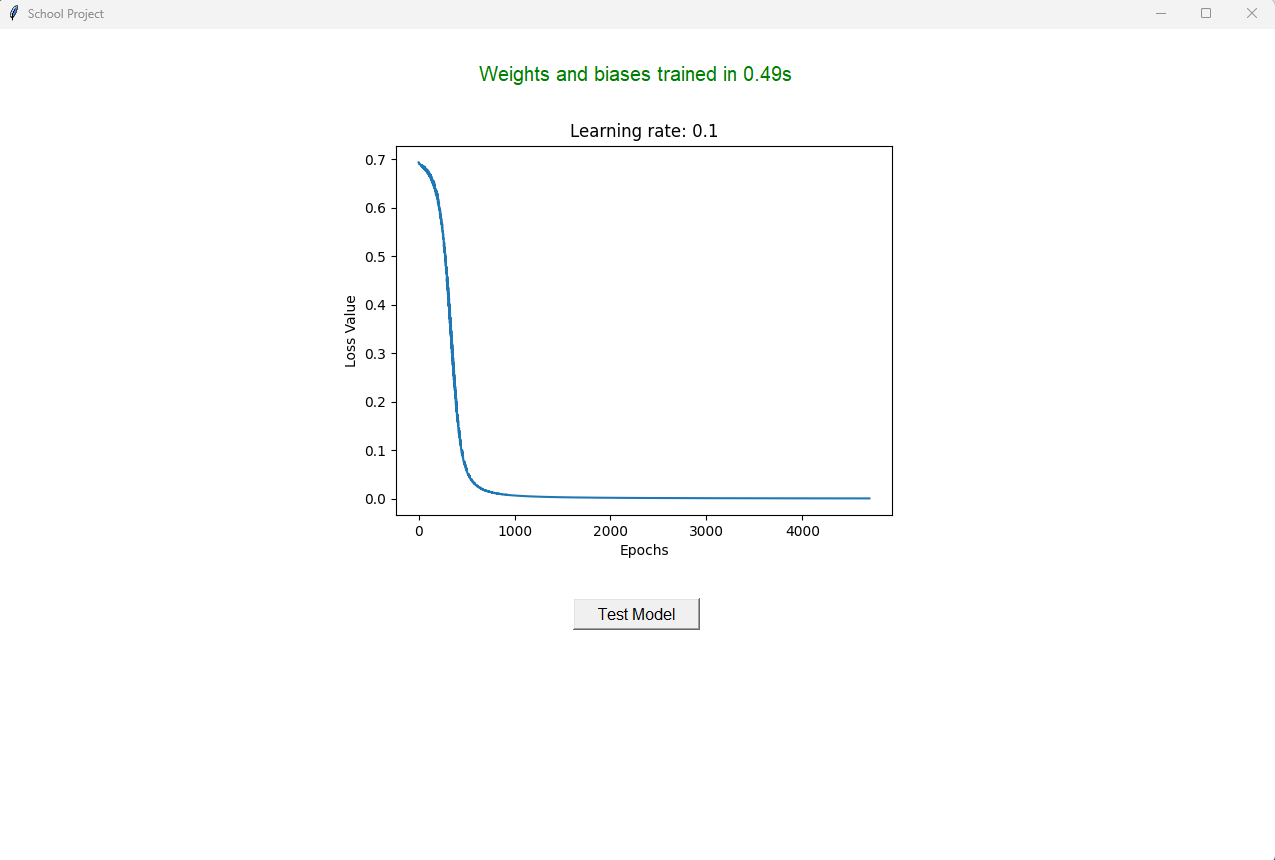
\includegraphics[width=1\textwidth]{./project-report/src/images/training-frame-2.png}}
        \end{figure}

    \item load\_model.py module:
        \inputminted{python}{./school_project/frames/load_model.py}

        Which outputs the following for the load model frame when models have been saved for the dataset:

        \pagebreak

        \begin{figure}[h!]
        \centering
        \frame{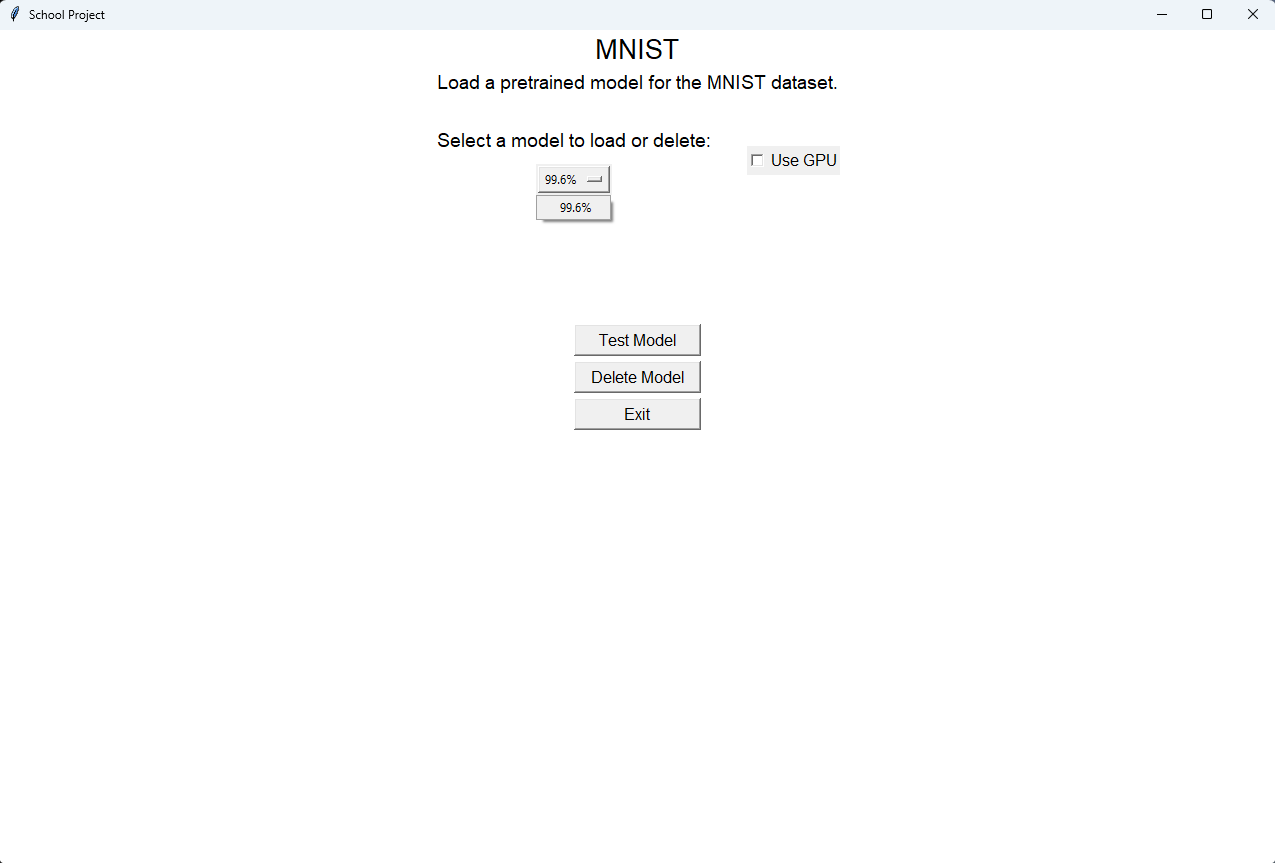
\includegraphics[width=1\textwidth]{./project-report/src/images/load-model-frame-1.png}}
        \end{figure}

        And outputs the following for the load model frame when no models have been saved for the dataset:

        \begin{figure}[h!]
        \centering
        \frame{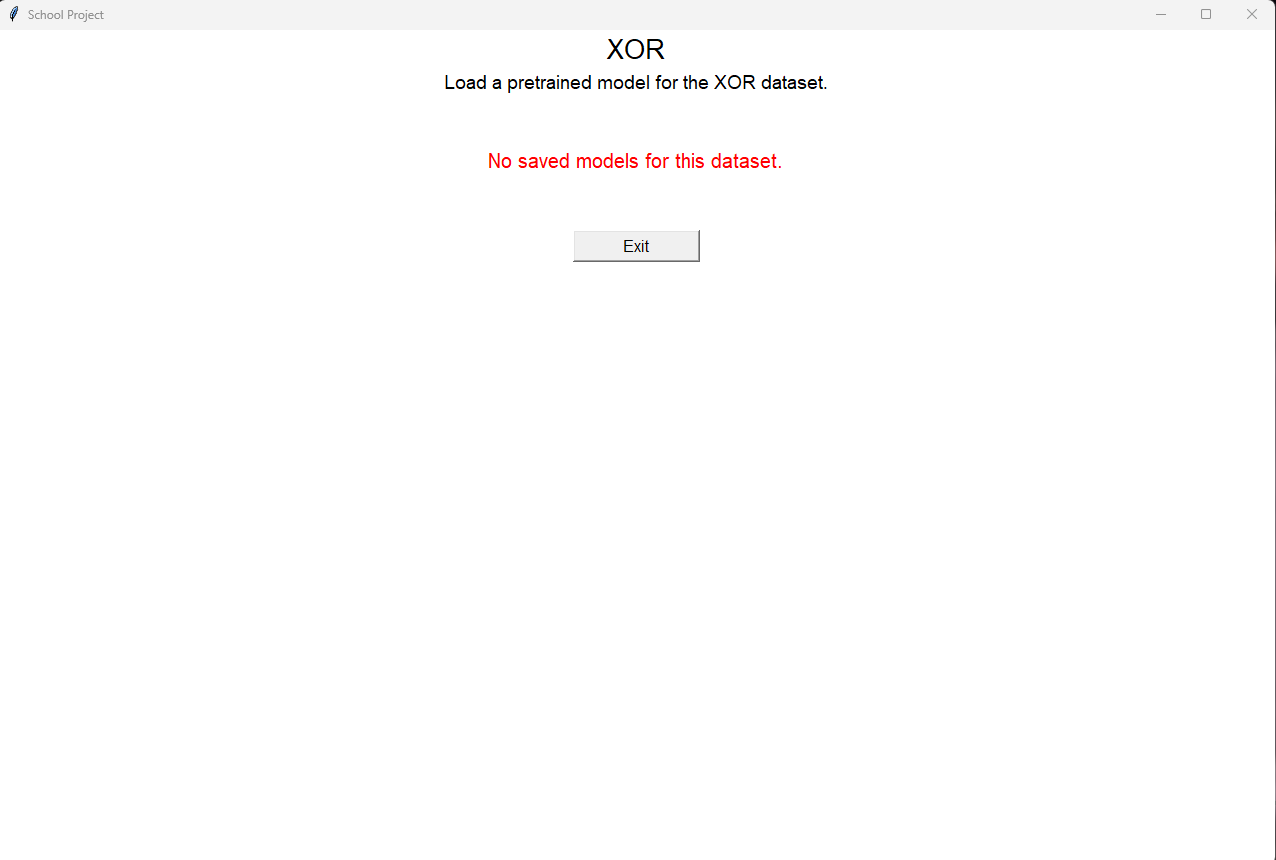
\includegraphics[width=1\textwidth]{./project-report/src/images/load-model-frame-2.png}}
        \end{figure}
\end{itemize}

\subsection{\_\_main\_\_.py module}

This module is the entrypoint to the project and loads the main window of the User Interface:

\inputminted{python}{./school_project/__main__.py}

Which outputs the following for the home frame:

\begin{figure}[h!]
\centering
\frame{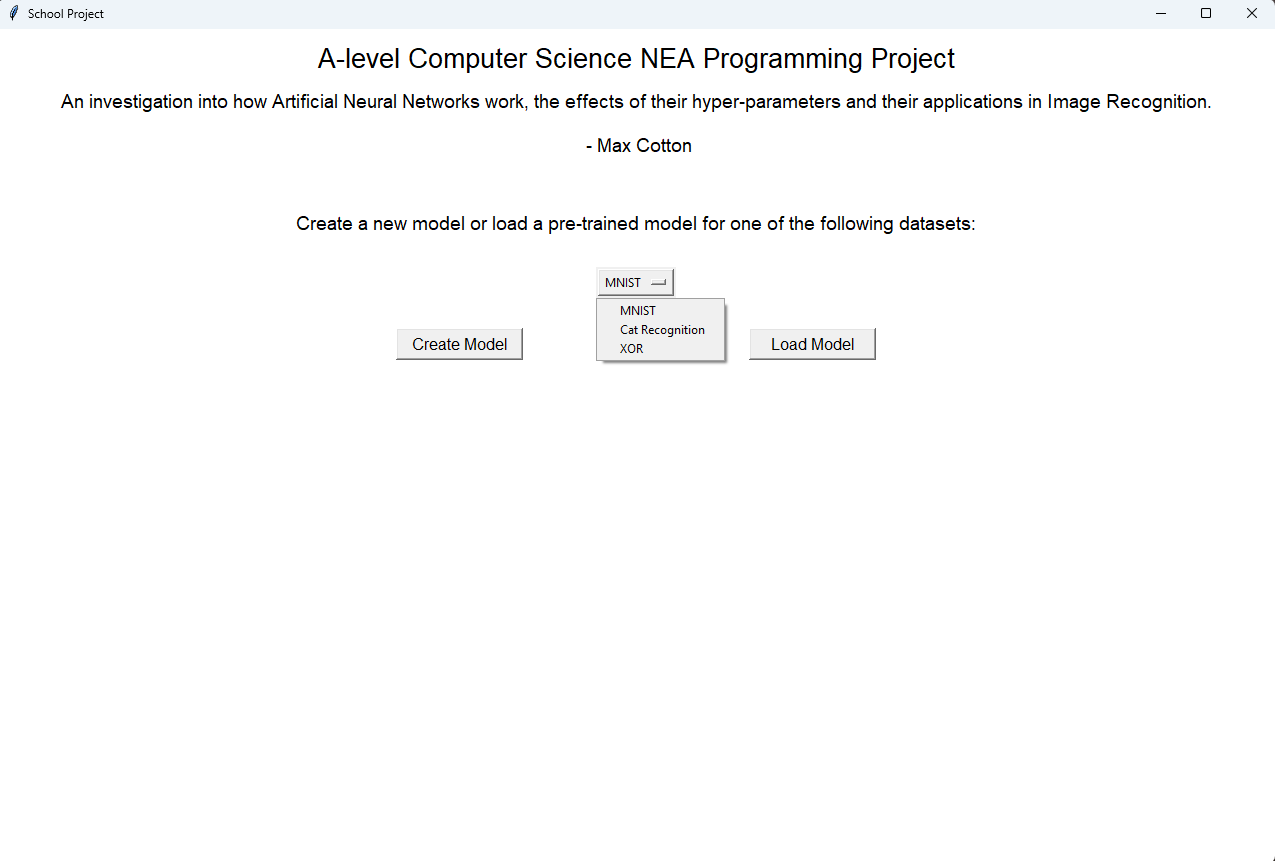
\includegraphics[width=1\textwidth]{./project-report/src/images/home-frame.png}}
\end{figure}

\end{document}